\chapter{Data Science in datengesteuerten Organisationen}

Inhalt dieses Kapitels ist die Darstellung des aktuellen Stands der Forschung zur Eingliederung von Data Science Teams in datengesteuerten Organisationen.
Damit wird verfolgt, ein aktuelles Zielbild annäherungsweise zu konkretisieren, um in weiteren Kapiteln auf die Möglichkeiten zur Integration einzugehen.

Eine Herausforderung entsteht bereits dabei, dass datengesteuerte Organisationen, in der Fachsprache als \textit{data driven Organizations} bezeichnet, einer Vielfalt an Definitionen unterliegen. \footcite[Vgl.][S. 4]{Dalpiaz.2020}
\Citeauthor*{Fabijan.2017} definierte z. B., dass datengesteuerte Organisationen Daten akquirieren, verarbeiten und Datenvorteile in einer zeitlich angebrachten Art und Weise nutzen, um Effizienzgewinne zu erzeugen, neuartige Produkte zu entwickeln und sich durch die Wettbewerbslandschaft zu navigieren. % \footcite[Vgl.][S. ]{Patil.2011}
% insert second definition
Ein gemeinsames Verständnis der Definitionen besteht in dem Prozess des Sammeln von Daten, der Gewinnung von Erkenntnissen durch Analysen und dem Treffen von Entscheidungen basierend auf den erzielten Analyseergebnissen. \footcite[Vgl.][S. 4]{Dalpiaz.2020}
Einer der wichtigsten Aspekte einer datengesteuerten Organisation ist die Manifestation einer datengesteuerten Kultur. \footcite[Vgl.][S. 15]{Dalpiaz.2020}
Dessen Antrieb ist es, Daten nicht nur den Analytic-Abteilungen oder dem leitenden Management vorbehalten sind, sondern so weit wie rechtlich möglich, jedem Organisationsmitglied zur Verfügung gestellt werden sollte. \footcite[Vgl.][S. 6]{Patil.2011}
Dieser Umgang würde es ermöglichen, alle Arten der Analyse (deskriptiv, prädiktiv, präskriptiv) auf allen Ebenen der Organisation (operativ, taktisch, strategisch) einzusetzen. \footcite[Vgl.][S. 4]{Dalpiaz.2020}
In der bisherigen Praxis wird von diesen Möglichkeiten jedoch nur ein Teil angewendet. \footcite[Vgl.][S. 4]{Dalpiaz.2020}
Weitere Aspekte einer datengesteuerten Organisation konnten durch die Forschung von \Citeauthor*{MariusHupperz.2021} identifiziert werden.
Für den untersuchten Aspekt der Data Science ist erkannt worden, dass der Wertbeitrag durch Transparenz, zielgerichtetem Marketing oder automatisierten informierten Entscheidungen zu Wettbewerbsvorteilen führen kann, jedoch keinen unmittelbaren Einflüsse auf die Vermögenswerte ausüben. \footcite[Vgl.][S. 5]{MariusHupperz.2021}
Zusätzlich kann Einrichtung einer Digitalisierungsabteilung zwar die Transformation zum datengesteuerten Unternehmen unterstützen, jedoch durch das alleinige Einrichten von Data Science Abteilungen keine Geschäftserkenntnisse aus Daten zu erzeugen. \footcite[Vgl.][S. 5]{MariusHupperz.2021}
Alle weiteren Aspekte aus der strukturierten Literaturanalyse von datengesteuerten Organisationen sind in folgender Abbildung 3.1 dargestellt:\footcite[Vgl.][S. 4]{MariusHupperz.2021}

\begin{figure}[htb]
    \centering
    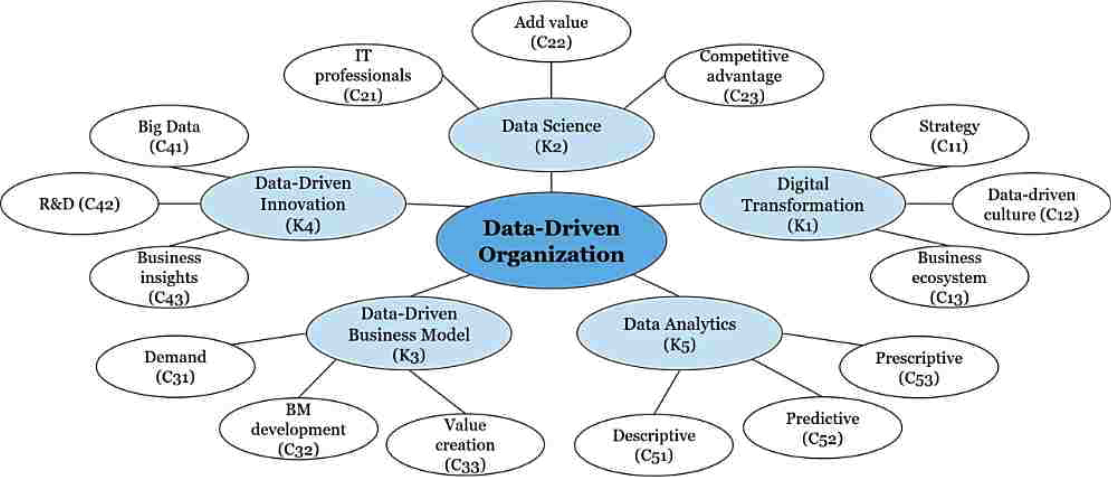
\includegraphics[width=0.95\textwidth]{graphics/ddo aspects.png}
    \caption{In der Literatur beschriebene Aspekte von datengesteuerten Organisationen}
    \label{fig:DDOs aspects}
\end{figure}

Zur praktischen Umsetzung von datengesteuerten Unternehmen führten \Citeauthor*{Zhang.2020b} eine Online Befragung mit insgesamt 183 Teilnehmenden aus der Data Science durch.
Da alle Beteiligten der Umfrage aus dem IT-Konzern IBM stammen, ist die Umfrage zwar nicht statistisch repräsentativ für alle Organisationen, zeigt jedoch ein signifikantes Bild über den Aufbau und die Zusammenarbeit von Data Science Abteilungen.
Mit der Umfrage sind Erkenntnisse sind erzielt worden, welche die fachliche, personelle und rollenbezogene Zusammensetzung und Zusammenarbeit von Data Science Abteilungen betreffen.
Ein Ergebnis der Umfrage ist es, dass Data science Abteilungen häufig mit einer Teamgröße von bis zu sechs Personen arbeiten, wobei jede Person bis zu 5 Jahre Erfahrung mit Data Science Projekten aufweisen kann. \footcite[Vgl.][S. 7]{Zhang.2020b}
Dabei führen die Teammitglieder meistens mehr als eine Rolle aus, was aus der nachträglichen Abbildung 3.2 (a) hervorgeht: \footcite[Vgl.][S. 7]{Zhang.2020b}

\begin{figure}[h]
    \centering
    \begin{subfigure}[b]{0.45\textwidth}
      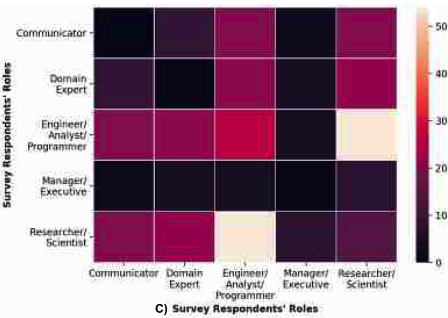
\includegraphics[width=\textwidth]{graphics/ds team roles.png}
      \caption{Häufigkeit der gemeinsam auftretenden Rollen in Data Science Teams}
      \label{fig:heatmap roles}
    \end{subfigure}
    \hfill
    \begin{subfigure}[b]{0.45\textwidth}
      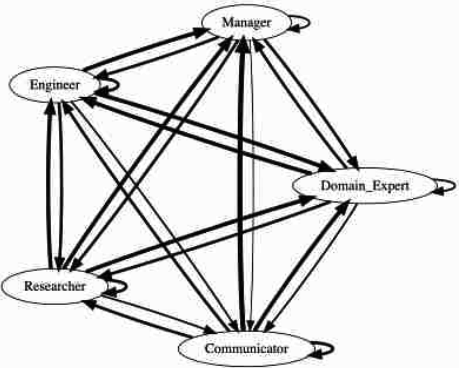
\includegraphics[width=\textwidth]{graphics/ds team network .png}
      \caption{Beziehungsgraph der Zusammenarbeit einzelner Rollen in Data Science Teams}
      \label{fig:network graph}
    \end{subfigure}
    \caption{Rollen und deren Zusammenarbeit in Data Science Teams}
    \label{fig:both_figures}
\end{figure}

Aus der Heatmap wird deutlich, dass die Kombination der Rollen \textit{Researcher - Engineer} am Häufigsten auftritt.
Dies resultiert vermutlich daraus, dass sich in der recht jungen Disziplin der Data Science noch wenig Standards etablierten, wodurch viele Konzepte in Projekten erstmalig zu entwickeln sind.
Durch die Diagnole der Abbildung, in welcher die Häufigkeit von einzeln vorkommenden Rollenbesetzungen abgetragen ist, wird ersichtlich, dass die \textit{Engineer} Rolle häufiger als alle anderen von einer Person ausgefüllt wird.
Daraus lässt sich vermuten, dass der hohe Entwicklungsaufwand in Data Science Projekten die Fokussierung von Personal zur \textit{Engineer} Rolle rechtfertigt.
Als Person in der Rolle des Managers werden, mit Ausnahme der \textit{Researcher} Rolle, noch seltener weitere Rollen ausgeübt, jedoch auch selten lediglich Aufgaben der eigenen Rolle übernommen.
Begründbar erscheint dies durch die Annahme, dass das Management häufig Aufgaben außerhalb des direkten Geschehens im Data Science Projekt umfasst.
Die Ausnahme der \textit{Researcher} Rolle würde sich logisch durch den gemeinsamen hohen Bedarf an Arbeitserfahrung im Themenfeld begründen lassen.

Abbildung 3.2 (b) zeigt den Umfang der Zusammenarbeit zwischen den verschiedenen Rollen auf.
Auffälligkeiten in der Grafik umfassen die Rolle des \textit{Communicators} und des \textit{Domain Experts}.
Die Rolle des \textit{Communicators} wird dabei vermutlich häufig sehr extrovertiert gestaltet, da hier besonders viel ausgehende Zusammenarbeit zu den anderen Rollen erkennbar ist, im Vergleich zu dessen Abhängigkeit.
Etwas gegensätzlich dazu zeigt sich die Rolle des \textit{Domain Experts}, welcher eine starke Abhängigkeit anderer Rollen abbildet, obwohl dabei wesentlich weniger technische Expertise zu erwarten ist.

% anschließend die Collaboration Points anbringen
In datengesteuerten Organisationen gilt es für eine Data Science Abteilung nicht nur innerhalb von sich selbst zusammenzuarbeiten, sondern auch z. B. Komponenten für maschinelles Lernen mit anderen Stakeholdern nutzbar zu gestalten.
Dazu sind vielerlei Punkte in der Abstimmung beider Teams notwendig, wie bspw. Anforderungserhebung, Trainingsdaten und Modellintegration, dessen bewährte Praktiken nachfolgend detaillierter betrachtet werden.
% requirement definition
In der anfänglichen Phase der Anforderungserhebung ist es zum einen wichtig Data Scientists früh in die Definition der Produktanforderungen einzubinden, jedoch zum anderen die Anforderungen an das zu entwickelnde Modell nicht losgelöst des Produkts zu betrachten. \footcite[Vgl.][S. 418]{Nahar.2022}
Die Zusammenarbeit kann zusätzlich unterstützt werden, indem zum einen technische Schulungen für Stakeholder wie Kunden, Produktteams und Endnutzer eingerichtet werden und zum anderen das gemeinsame Verständnis der Anforderungen bestmöglich dokumentiert wird. \footcite[Vgl.][S. 418]{Nahar.2022}
% training data 
Während der Abstimmung der Trainingsdaten mit anderen Abteilungen profitiert der Projektfortschritt, wenn Data Science Teams die Freiheit besitzen, Erwartungen bezüglich z. B. Datenqualität an Lieferanten zu stellen. \footcite[Vgl.][S. 420]{Nahar.2022}
Sollte aufgrund der Projekt- oder Organisationsgröße eine direkte Zusammenarbeit mit dem Datenlieferanten nicht umsetzbar sein, bleibt es notwendig, entsprechende Erwartungen in formalen Verträgen festzuhalten. \footcite[Vgl.][S. 420]{Nahar.2022}
% product model integration
Nach den bisherigen Abstimmung und der Entwicklung des Produkts bleibt der kontinuierliche Prozess des Betriebs.
Die Qualitätssicherung spielt in dieser Phase eine signifikante Rolle und sollte geplant und mit Schulungen zu Themen wie \textit{DevOps} und \textit{MLOps} unterstützt werden. \footcite[Vgl.][S. 423]{Nahar.2022}

Folgend werden Herausforderungen und Vorgehen behandelt, wie eine Transformation zur datengesteuerten Organisation gelingt, sodass Geschäftsmehrwert aus solcher Arbeit entsteht.
